\documentclass{beamer}
\setbeamertemplate{caption}[numbered]
\usepackage{graphicx}
\usepackage{svg}
\usepackage[utf8]{inputenc}
\usepackage[english]{babel}
\graphicspath{{Graphs/}}
\usepackage{comment}
\usepackage{verbatim}
\usepackage{hyperref}
\mode<presentation>
{
	\usetheme{AnnArbor}
	\usecolortheme{crane}
}

\title[Model Interpretation and Visualization using Stata]{Model Interpretation and Visualization using Stata}
\subtitle[ISRC Workshop]{Iowa Social Research Center (ISRC) Workshop}
\author[Wallace]{Desmond D. Wallace}
\institute[University of Iowa]{Department of Political Science\\The University of Iowa\\Iowa City, IA}

\date{November 17, 2017}

\begin{document}

\begin{frame}
 \titlepage
\end{frame}

%\begin{frame}
%	\frametitle{Table of Contents}
%	\tableofcontents
%\end{frame}

\section{Regression Basics}

\begin{frame}
	\frametitle{Regression Highlights}
	\begin{itemize}
		\item A way to summarize the relationship between variables.
		\item Assuming there is a relationship between Y and the independent variable(s).
		\item Relationship may be linear (OLS) or non-linear (CLDV).
		\item \textbf{Regression helps our understanding of how our dependent variable of interest changes when one or more independent variables vary, while holding remaining variables fixed.}
	\end{itemize}
\end{frame}

\section{Reporting Regression Results}
\subsection{Tables}

\begin{frame}
	\frametitle{Regression Tables}
		\begin{itemize}
			\item Important to report regression results in publication quality
			\item NEVER USE STATA output
			\item Multiple ways to create tables that can be featured in Word,PowerPoint,\LaTeX documents
			\item Information table should feature include:
				\begin{enumerate}
					\item Coefficient Estimate (REQUIRED)
					\item Standard Errors (Could include test statistic or $p$-value)
					\item Significance Stars
					\item Model Fit Statistics are useful (e.g., $R^2$)
				\end{enumerate}
		\end{itemize}
\end{frame}

\begin{frame}
	\frametitle{\texttt{outreg2}}
		\begin{itemize}
			\item \texttt{outreg2} is a user-written Stata program
			\item Provides a fast and easy to produce regression tables
			\item Basic Syntax: \texttt{outreg2 using \textit{filename}, replace}
			\item \texttt{outreg2} command is executed AFTER regression model is estimated
		\end{itemize}
\end{frame}

\begin{frame}
	\frametitle{\texttt{outreg2} Example}
		\texttt{reg realrinc age i.female}\\
		\texttt{outreg2 using Tables/model.tex, replace tex(fragment)}
\end{frame}

\begin{frame}
	\frametitle{\texttt{outreg2} Example}
		\begin{tabular}{lc} \hline
 & (1) \\
VARIABLES & realrinc \\ \hline
 &  \\
age & 255.8*** \\
 & (39.38) \\
Constant & 9,558*** \\
 & (1,807) \\
 &  \\
Observations & 1,201 \\
 R-squared & 0.034 \\ \hline
\multicolumn{2}{c}{ Standard errors in parentheses} \\
\multicolumn{2}{c}{ *** p$<$0.01, ** p$<$0.05, * p$<$0.1} \\
\end{tabular}

\end{frame}

\subsection{Plots}

\begin{frame}
	\frametitle{Coefficient Plots}
		\begin{itemize}
			\item Sometimes, regression models feature many variables
			\item Also, showing many numbers and stars can be difficult for some readers
			\item An alternative to reporting a table is a plot of the regression results
		\end{itemize}
\end{frame}

\begin{frame}
	\frametitle{\texttt{coefplot}}
		\begin{itemize}
			\item \texttt{coefplot} is another user-written Stata program
			\item Plots regression results in ``dot-whisker" format
				\begin{itemize}
					\item ``Dot" -- Coefficient Estimate
					\item ``Whisker" -- Confidence Interval
				\end{itemize}
			\item Basic Syntax: \texttt{coefplot}
			\item \texttt{coefplot} command is executed AFTER regression model is estimated
		\end{itemize}
\end{frame}

\begin{frame}
	\frametitle{\texttt{coefplot} Example}
		\texttt{reg realrinc age i.female}\\
		\texttt{coefplot}
\end{frame}

\begin{frame}
	\frametitle{\texttt{coefplot} Example}
		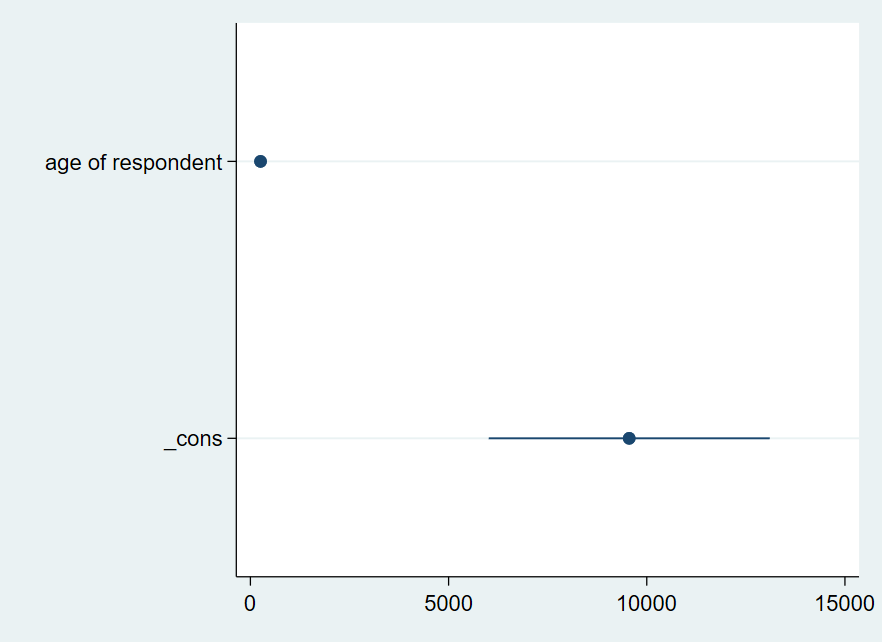
\includegraphics[scale=0.3]{coefplot.png}
\end{frame}

\begin{frame}
	\frametitle{\texttt{coefplot} Example}
		\texttt{reg realrinc age i.female}\\
		\texttt{coefplot, drop(\_cons)}
\end{frame}

\begin{frame}
	\frametitle{\texttt{coefplot} Example}
		%\includegraphics[scale=0.3]{coefplotDrop.png}
\end{frame}

\section{Interpretation}
\subsection{Coefficients}

\begin{frame}
	\frametitle{Interpreting Coefficients}
		\begin{itemize}
			\item Can directly interpret coefficient estimates.
			\item \textit{A one unit change in $X_{k}$ leads to a $\beta_{k}$ change in $Y$ (holding all other variables constant).}
			\item Assumes $X_{k}$ is not a constituent term for an interaction variable. 
		\end{itemize}
\end{frame}

\subsection{Predicted (Fitted) Values}

\begin{frame}
	\frametitle{Predicted (Fitted) Values}
		\begin{itemize}
			\item The result of substituting values of interest for the independent variable(s).
			\item $E[Y|X]=X\hat{\beta}$
			\item Can calculate standard errors to determine if $E[Y|X=x]$ is statistically significantly different from zero.
			\item Multiple ways to calculate fitted values in Stata.
		\end{itemize}
\end{frame}

\subsection{Marginal Effects}

\begin{frame}
	\frametitle{Marginal and Discrete Change}
		\begin{itemize}
			\item Measuring the change in the dependent variable for a change in one independent variable, holding remaining independent variables constant.
				\begin{itemize}
					\item \textit{Marginal Change} is the partial derivative, or instantaneous rate of change, in the dependent variable w.r.t. an independent variable, holding remaining variables constant.
					\item \textit{Discrete Change} or \textit{First Difference} is the difference in the prediction from one specified value of an independent variable to another specified value, holding remaining variables constant.
				\end{itemize}
		\end{itemize}
\end{frame}

\begin{frame}
	\frametitle{Marginal and Discrete Change}
		\begin{itemize}
			\item Marginal Change: $\frac{\partial E[Y|X]}{\partial x_{k}}=\frac{\partial X\beta}{\partial x_{k}}=\beta_{k}$
			\item Discrete Change: $\frac{\Delta E[Y|X]}{\Delta x_{k}}=E[Y|X, x_{k}+1]-E[Y|X, x_{k}]=\beta_{k}$
		\end{itemize}
\end{frame}

\begin{frame}
	\frametitle{Marginal and Discrete Change}
		\begin{itemize}
			\item $\frac{\partial E[Y|X]}{\partial x_{k}}=\frac{\Delta E[Y|X]}{\Delta x_{k}}=\beta_{k}$, assuming there is no interaction terms.
			\item The standard error of the marginal effect is the same as the standard error of the estimated beta coefficient.
			\item \textit{For a unit increase in $x_{k}$, the expected change in $Y$ equals $\beta_{k}$, holding all other variables constant.}
			\item \textit{Having characteristic $x_{k}$ (as opposed to not having the characteristic) results in an expected change of $\beta_{k}$ in $Y$, holding all other variables constant.}
			\item When there is no interaction term present, $\mbox{Marginal Change}=\mbox{Discrete Change}$
		\end{itemize}
\end{frame}

\begin{frame}
	\frametitle{Marginal Effects}
		%\begin{figure}[p]
		%	\centering
		%	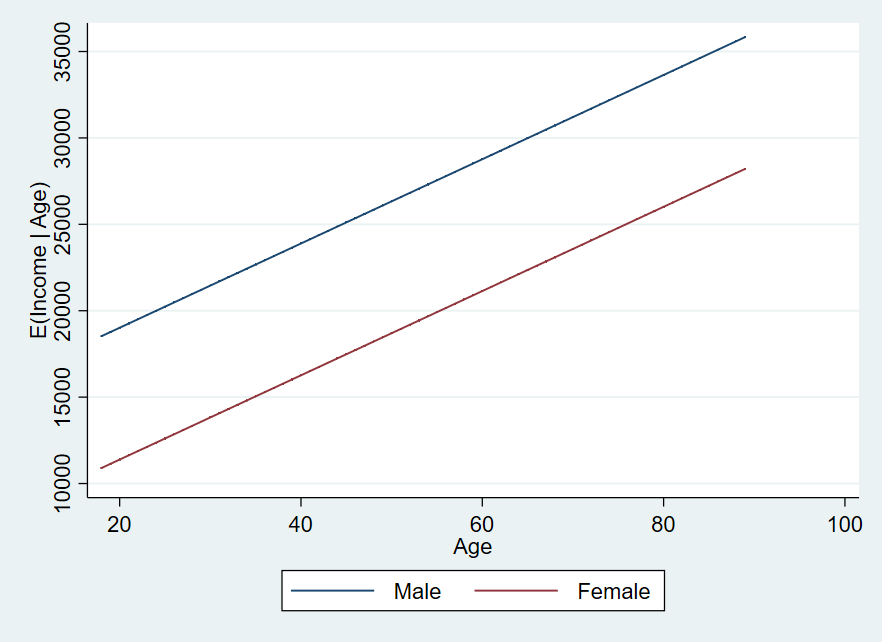
\includegraphics[width=1\textwidth]{Graphs/mfxOLS.png}
		%	\label{fig:fig1}
		%\end{figure}
\end{frame}

\section{\texttt{margins} and \texttt{marginsplot}}
\subsection{\texttt{margins}}

\begin{frame}
	\frametitle{\texttt{margins}}
	\begin{itemize}
		\item Computes predicted values and marginal effects from last estimated regression model
		\item Reports computed statistic, standard error, test statistic, $p$-value and 95\% CI.
		\item \texttt{at(atspec)} option allows for the calculation of predicted values and marginal effects at specific values of independent variable(s).
		\item \texttt{dydx()} option allows for calculating marginal effects.
		\item Factor variables (\texttt{i.\underline{varname}}) can go after the \texttt{margins} command or within the \texttt{at(atspec)} option.
		\item Continuous variables can only be specified within the \texttt{at(atspec)} option.
		\item \texttt{atmeans} option sets variables not specified to be held at their mean value.
	\end{itemize}
\end{frame}

\begin{frame}
	\frametitle{Predicted (Fitted) Values -- \texttt{margins} Syntax}
		\begin{itemize}
			\item \texttt{margins} -- Overall predicted value with all independent variables held at their mean value.
			\item \texttt{margins, at(varname=\#)} -- Predicted value when one or more independent variables are fixed to a specific value and remaining independent variables held at their mean value.
			\item \texttt{margins, at(varname=numlist)} -- Predicted value(s) when one or more independent variables are fixed to multiple values and remaining independent variables held at their mean value.
			\item \texttt{margins varname} -- Overall predicted value(s) for categories of \texttt{varname} with remaining independent variables held at their mean value.
		\end{itemize}
\end{frame}

\begin{frame}
	\frametitle{Marginal Change -- \texttt{margins} Syntax}
		\begin{itemize}
			\item \texttt{margins, dydx(varname)} -- Average marginal effect a one-unit increase in \texttt{varname} has on the dependent variable, holding all other variables constant.
		\end{itemize}
\end{frame}

\begin{frame}
	\frametitle{Discrete Change -- \texttt{margins} Syntax}
		\begin{itemize}
			\item \texttt{margins, at(varname=(\textit{start} \textit{end})) post} -- Calculates predicted values at specified values, and treats results as estimation results.
			\item \texttt{lincom $\mbox{2.\_at}-\mbox{1.\_at}$} -- Calculates the difference between the prediction of the ending value and the prediction of the starting value.
		\end{itemize}
\end{frame}

\subsection{\texttt{marginsplot}}

\begin{frame}
	\frametitle{\texttt{marginsplot}}
	\begin{itemize}
		\item Graphs the results of last estimated \texttt{margins} command
		\item \textbf{Needs to be executed immediately after \texttt{margins}}
		\item Resulting graph includes an overall title, a title for the $y$-axis, $x$-axis features the name of the variable (variable label if one is included).
		\item The featured values on the $x$-axis are the values specified from the \texttt{margins} command.
		\item Can use the \texttt{recast} and \texttt{recastci} options to change how results are graphed.
	\end{itemize} 
\end{frame}

\begin{frame}
	\begin{center}
		\begin{LARGE}
			Email: desmond-wallace@uiowa.edu\\
			Any Questions?
		\end{LARGE}
	\end{center}
\end{frame}

\end{document}
